\documentclass{article}
\usepackage{graphicx}
\usepackage[margin=1.5cm]{geometry}
\usepackage{amsmath}

\begin{document}

\title{Tuesday Reading Assessment: Unit 0 part II, Capacitance}
\author{Prof. Jordan C. Hanson}

\maketitle

\section{Memory Bank}

\begin{itemize}
\item $Q = CV$ ... Relationship between capacitance, charge, and voltage.
\item $C_{tot} = C_1 + C_2 + C_3 + ...$ ... Capacitors in parallel.
\end{itemize}

\section{Capacitors}

\begin{enumerate}
\item Consider Fig. \ref{fig:plates}.  Why does each capacitor add to the total capacitance if each is connected to the battery as shown?  What physical principles are working here? \\ \vspace{1.5cm}
\begin{figure}[ht]
\centering
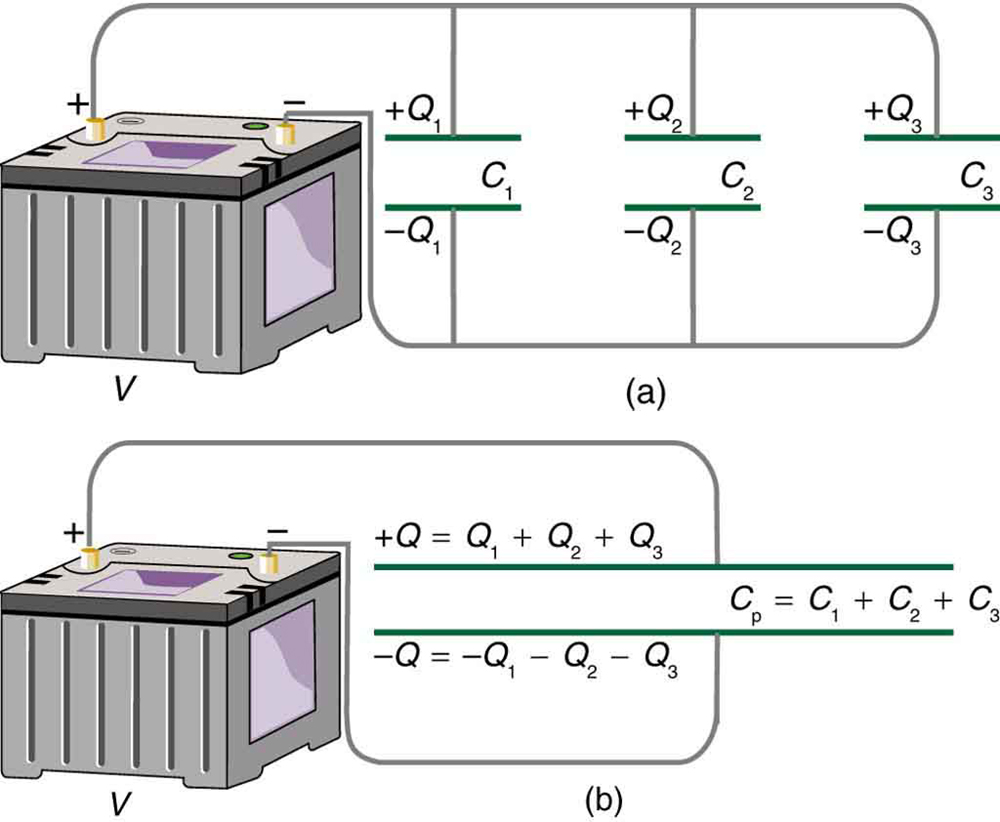
\includegraphics[width=0.3\textwidth]{cap1.jpeg}
\caption{\label{fig:plates} The relationship between potential energy and voltage.}
\end{figure}
\item Suppose $C_1$ is 20 pF, $C_2$ is 20 pF, and the total capacitance is 100 pF.  What is the capacitance of $C_3$? \\ \vspace{1cm}
\item Suppose the total charge stored is 1 pC, and the total capacitance is 24 pF.  At what voltage is the charge being stored? \\ \vspace{1cm}
\item Suppose a different system stores the same charge at half the voltage.  What is true of the capacitance?
\begin{itemize}
\item A: It has half the capacitance
\item B: It is the same capacitance
\item C: It is double the capacitance
\item D: It has zero capacitance
\end{itemize}
\end{enumerate}

\end{document}
